% =============================================================================
% Draft IEEE conference paper.
% Build:  pdflatex main && pdflatex main      (needs IEEEtran.cls; Overleaf has it)
% Every number below was produced by code in this repository (see the
% "Reproducibility" section). Items marked TODO are not yet measured.
% =============================================================================
\documentclass[conference]{IEEEtran}

\usepackage{cite}
\usepackage{amsmath,amssymb}
\usepackage{graphicx}
\usepackage{booktabs}
\usepackage{array}
\usepackage{url}
\usepackage{tikz}
\usetikzlibrary{arrows.meta,positioning,shapes.geometric,fit}

\def\BibTeX{{\rm B\kern-.05em{\sc i\kern-.025em b}\kern-.08em
    T\kern-.1667em\lower.7ex\hbox{E}\kern-.125emX}}

\begin{document}

\title{Speaker-Independent Verbatim Transcription of Overlapping Meeting Speech with Near-Real-Time Streaming on Consumer Hardware}

\author{\IEEEauthorblockN{Shreya Mary Kurien, Krishiv Saluja, Sampath Bageyawadi, Thummala Koushik, M Sanjay}
\IEEEauthorblockA{Department of Computer Science and Engineering\\
Woxsen University, Hyderabad, India}}

\maketitle

\begin{abstract}
Transcribing a conversation recorded by a single microphone in a room requires solving four problems at once: deciding who is speaking, recovering speech that overlaps, keeping disfluencies such as ``um'' and ``uh'' that off-the-shelf recognisers delete, and doing all of this quickly enough to be useful live. We describe a modular pipeline that combines neural diarisation, overlap-aware routing, two-source speech separation with voice-based stream-to-speaker assignment, and verbatim Whisper recognition, and a streaming variant that keeps speaker labels stable over a sliding window. On an Apple M3 laptop, moving Whisper-small from CPU to the Apple GPU (MLX) made transcription $5.2\times$ faster with an identical transcript, and together with GPU diarisation, clip packing and label stabilisation reduced end-to-end streaming latency from a mean of 14.5\,s (growing) to about 7--8\,s (bounded) on a two-speaker test. We also fine-tune Whisper-small on 20.2 hours of far-field AMI meeting audio, training only the top two encoder layers and the decoder from cached encoder activations so that it fits on a 17\,GB machine. On held-out meetings, filler recall rises from 0/96 (utterance-level) and 2/83 (full-pipeline meeting excerpts) to 74\% and 83\% respectively, but word error rate on raw single-microphone clips worsens (38.8\% to 42.5\%) because the model transcribes all audible speech, not only the labelled speaker. In full-pipeline scoring of three four-person AMI excerpts the fine-tuned recogniser is slightly worse on concatenated-permutation WER (mean 57.1\% vs.\ 55.5\%, mixed across meetings) at a mean DER of 19.4\%. Our evaluation is small-scale and partly synthetic, and we state its limits explicitly.
\end{abstract}

\begin{IEEEkeywords}
speaker diarization, speech separation, overlapped speech, verbatim ASR, disfluency, streaming, Whisper, AMI
\end{IEEEkeywords}

%% ---------------------------------------------------------------------------
\section{Introduction}
Meeting transcription from a shared room microphone is difficult for reasons that compound. Speakers talk over each other; the recogniser must attribute words to the right person; and downstream users of a transcript (minute takers, researchers studying conversation, accessibility tools) often need the speech as it was said, including fillers, repetitions and pauses. Large weakly supervised recognisers such as Whisper~\cite{radford2023whisper} are strong general-purpose transcribers but are trained to produce clean text: on far-field meeting speech they routinely delete fillers and backchannels. Conversely, systems built for overlapped speech typically target a fixed evaluation setup and are not designed to run live on a personal computer.

This paper describes an end-to-end pipeline, and reports what we measured while building it, with three aims: (i) speaker independence, meaning it works for an arbitrary set of speakers with no per-speaker training and only optional enrolment for real names; (ii) verbatim output; and (iii) near-real-time streaming on consumer hardware. Our contributions are:
\begin{itemize}
\item A modular pipeline in which overlap flags and speech boundaries are derived from a single diarisation pass, overlapped segments are separated by a two-source model, and separated streams are mapped back to diarised speakers by voice similarity, which is necessary because separator output order is arbitrary (Sec.~\ref{sec:system}).
\item A streaming variant with a session-long speaker registry that stabilises \texttt{Speaker\_N} labels using temporal continuity between overlapping windows and voice similarity only as a fallback (Sec.~\ref{sec:streaming}).
\item Engineering measurements that determined whether the system runs live: an Apple-GPU Whisper backend, a cost model showing Whisper call time is independent of clip length, and packing of clean clips into shared 30\,s windows, including a case where packing hurt accuracy (Sec.~\ref{sec:latency}).
\item A memory-lean recipe for adapting Whisper-small to verbatim far-field meeting speech on a 17\,GB laptop, and an honest analysis of its mixed outcome (Sec.~\ref{sec:finetune}).
\end{itemize}

%% ---------------------------------------------------------------------------
\section{Related Work}
\textbf{Diarisation.} pyannote.audio~\cite{bredin2023pyannote} provides a segmentation-plus-clustering pipeline whose frame-level segmentation network handles overlapped speech~\cite{plaquet2023powerset}; we rely on its output turns, which preserve simultaneous speakers, rather than running a separate voice-activity or overlap detector.

\textbf{Separation.} SepFormer~\cite{subakan2021sepformer} is a transformer separator trained on synthetic two-speaker mixtures (e.g.\ WSJ0-2mix, Libri2Mix~\cite{cosentino2020librimix}). Such models are permutation-ambiguous; utterance-level permutation training fixes the order within a segment but not across segments, which is why streams must be re-associated with speakers in a continuous pipeline. Continuous separation benchmarks such as LibriCSS~\cite{chen2020libricss} evaluate this setting.

\textbf{Multi-speaker ASR evaluation.} The CHiME challenges~\cite{watanabe2020chime6} popularised concatenated minimum-permutation WER (cpWER), which penalises both wrong words and words credited to the wrong speaker; we use it together with diarisation error rate (DER).

\textbf{Meeting corpora.} The AMI corpus~\cite{carletta2005ami} contains scenario and non-scenario meetings recorded with individual headsets and with distant microphone arrays, with verbatim transcripts that retain disfluencies. We use its single-distant-microphone (SDM) condition, the closest public match to a phone or laptop on a table.

%% ---------------------------------------------------------------------------
\section{System}\label{sec:system}
Fig.~\ref{fig:arch} shows the pipeline. All models are open-weight and run locally.

\begin{figure}[t]
\centering
\resizebox{0.92\columnwidth}{!}{%
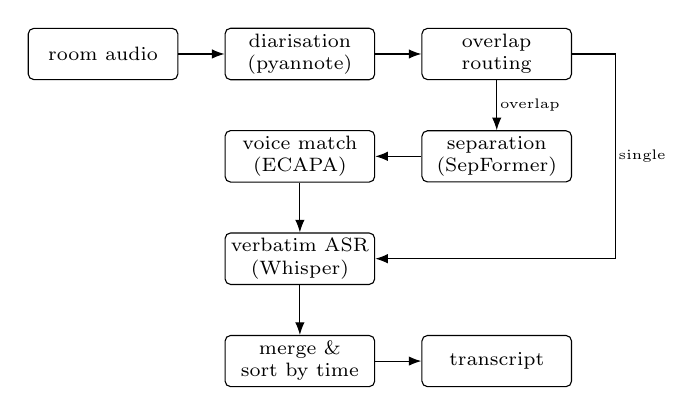
\begin{tikzpicture}[
  box/.style={draw, rounded corners=2pt, minimum height=6.5mm, minimum width=19mm, font=\scriptsize, align=center, inner sep=2pt},
  arr/.style={-{Latex[length=1.6mm]}, thin},
  lab/.style={font=\tiny, inner sep=1pt}]
  \node[box] (audio) at (0,0)      {room audio};
  \node[box] (diar)  at (2.5,0)    {diarisation\\(pyannote)};
  \node[box] (route) at (5.0,0)    {overlap\\routing};
  \node[box] (sep)   at (5.0,-1.3) {separation\\(SepFormer)};
  \node[box] (match) at (2.5,-1.3) {voice match\\(ECAPA)};
  \node[box] (asr)   at (2.5,-2.6) {verbatim ASR\\(Whisper)};
  \node[box] (merge) at (2.5,-3.9) {merge \&\\sort by time};
  \node[box] (out)   at (5.0,-3.9) {transcript};
  \draw[arr] (audio) -- (diar);
  \draw[arr] (diar) -- (route);
  \draw[arr] (route) -- node[right, lab]{overlap} (sep);
  \draw[arr] (sep) -- (match);
  \draw[arr] (match) -- (asr);
  \draw[arr] (route.east) -- ++(0.55,0) |- node[pos=0.25, right, lab]{single} (asr.east);
  \draw[arr] (asr) -- (merge);
  \draw[arr] (merge) -- (out);
\end{tikzpicture}}
\caption{Pipeline. Single-speaker segments go straight to recognition; overlapped segments are separated, each stream is matched to a diarised speaker by voice, then recognised. Lines are merged in time order.}
\label{fig:arch}
\end{figure}

\subsection{Diarisation and overlap routing}
We use the pyannote speaker-diarization-3.1 pipeline. Its turns keep simultaneous speakers as overlapping turns, so one pass yields both speech/non-speech boundaries and overlap flags. We cut the timeline at every turn boundary, label each piece with its set of active speakers, and merge neighbouring pieces with identical sets separated by at most 0.4\,s. Overlaps shorter than 0.4\,s are folded into the neighbouring speaker because SepFormer is unreliable on such short clips and they are typically backchannels or boundary jitter. The result is a list of segments $(t_s, t_e, \mathcal{S})$, treated as overlapping when $|\mathcal{S}|\ge 2$.

\subsection{Separation and stream-to-speaker assignment}
Overlapped segments are separated by a SepFormer checkpoint at 8\,kHz into two streams (resampling is handled internally). Both outputs are scaled by one shared factor so their relative levels are preserved; a stream whose RMS is below 10\% of the louder one is treated as leakage and skipped, since recognisers hallucinate words on such residue.

Because the output order is arbitrary, we compute for each diarised speaker a voice print from their \emph{clean} (non-overlapped) speech using ECAPA-TDNN~\cite{desplanques2020ecapa} embeddings (SpeechBrain~\cite{ravanelli2021speechbrain}), embed each separated stream, and solve a one-to-one assignment maximising total cosine similarity with the Hungarian algorithm. Speakers who never talk alone have no clean print; they are paired positionally with any unmatched stream as a last resort. Optional enrolment reuses the same embedder: an enrolled clip's embedding is matched to speaker prints above a threshold, replacing the generic label by a name.

\subsection{Verbatim recognition and boundary handling}
Whisper's default decoding suppresses a set of non-speech tokens, which we disable. Each segment is transcribed with 0.4\,s of extra context on both sides, and only words whose timestamp midpoint lies inside the segment are kept, so a word straddling a boundary is assigned to exactly one segment and none is chopped. For separated streams the crop is applied at an edge only when a neighbouring segment also transcribes the same speaker; otherwise a speaker who \emph{starts} inside the overlap would lose a first word whose timestamp Whisper stretches back into leading silence. Gaps between words of at least 0.6\,s are rendered as explicit pause markers. Decoding is greedy with a temperature fallback ($0, 0.2, 0.4$) when the output is repetitive (compression ratio above 2.4) or low-confidence; generation is capped at 8 tokens per second of audio plus 24, and a segment still above compression ratio 2.8 is dropped. On separated streams, utterances consisting only of fillers are discarded, because the fine-tuned model emits confident lone ``mm'' tokens on separation residue.

%% ---------------------------------------------------------------------------
\section{Streaming}\label{sec:streaming}
The streaming variant reuses every stage on a rolling buffer. Every $\ge$4\,s of new audio, the last 16\,s are re-diarised; only audio older than a 3\,s guard is \emph{committed}, so emitted lines are never retracted. The latency of a line is therefore roughly the guard plus processing time plus the wait for the next step. Steps run in a worker thread; a step never starts while another is running, so on slow hardware the hop grows instead of the system falling behind.

\textbf{Stable speaker labels.} Each window's diarisation produces arbitrary local labels. We map them to session-long identities with a registry of running voice prints, using two kinds of evidence in order of trust: (1) \emph{temporal continuity}: consecutive windows share most of their audio, so a local speaker active at the same moments as a previously labelled speaker inherits its label (Hungarian matching on overlapped seconds, minimum 0.4\,s); (2) \emph{voice similarity} against registered prints (cosine threshold 0.4) for speakers with no temporal anchor. Two safeguards mattered in practice. A print computed only from overlapped speech is marked \emph{weak}: it may create a provisional identity but never updates an existing speaker's print. A speaker present only inside the guard region is not registered at all until they appear in committed audio; without this, a phantom duplicate identity was created for a speaker whose first second fell in the unstable tail. A speaker-count hint is applied as an upper bound, since forcing an exact count on a short window makes the diarizer split one voice into two.

%% ---------------------------------------------------------------------------
\section{Verbatim Adaptation on AMI}\label{sec:finetune}
\subsection{Data}
We use the utterance-level AMI SDM release (CC BY 4.0), whose transcripts are verbatim (fillers such as \emph{um}, \emph{uh}, \emph{hmm}, \emph{mm-hmm} are kept, roughly 1 in 40 words). Utterances average 3\,s, but Whisper always encodes a padded 30\,s window, so training on single utterances wastes about 90\% of the compute and never exposes the model to multi-speaker windows. All clips of a meeting come from the same microphone, so we rebuild each meeting's timeline by placing clips at their start times and cut it into windows of up to 28\,s containing consecutive utterances, labelled in Whisper's native format with timestamp tokens (consecutive segments separated by an end/start timestamp pair), so segment and word timing keep working. Text is lower-cased without punctuation (AMI's own convention). Each window is loudness-normalised (RMS 0.05); the far-field audio is very quiet (peak $\approx 0.02$), and the same normalisation is applied at inference.

We use 7 of 27 training shards, chosen evenly across the split for meeting diversity: 3\,612 windows, 27\,725 utterances, 20.2\,h, 40 meetings. One validation shard (381 windows, 5 meetings) and two of four test shards are held out, with no meeting shared between splits. Evaluation uses 300 utterances sampled from the test meetings.

\subsection{Cached-encoder fine-tuning}
On the Apple M3 (MPS), for a batch of four 30\,s windows the Whisper-small encoder costs 2.81\,s forward+backward versus 0.46\,s for the decoder, so full fine-tuning would take about 4.5\,h per 1\,200 steps. We instead run the frozen lower ten encoder layers \emph{once} and cache the hidden states entering layer 10 as float16 (8.3\,GB for training), then train the top two encoder layers, the final encoder norm and the whole decoder (168\,M of 242\,M parameters) from the cache. The decoder learns the verbatim style and meeting vocabulary; the top encoder layers adapt to far-field acoustics. Training used AdamW, learning rate $10^{-5}$ with linear warm-up and decay, effective batch 8 (2 windows $\times$ 4 accumulation), and 1\,350 optimiser steps ($\approx$3 epochs). A micro-batch of 4 exhausted memory (GPU driver allocation grew from 5.0 to 8.4\,GB and the machine swapped), so we used 2. Training was interrupted once and resumed from the step-200 checkpoint with a fresh optimiser state and schedule, which we disclose as a deviation from a clean run. The fine-tuned weights are converted to MLX format; our converter reproduces the published stock MLX weights exactly (479 tensors, maximum difference 0) before being used on the fine-tuned model.

%% ---------------------------------------------------------------------------
\section{Experiments}\label{sec:exp}
\textbf{Setup.} All timing is on one Apple M3 with 17\,GB unified memory. Software: PyTorch 2.14, pyannote.audio 4.0.7, SpeechBrain 1.1.1, faster-whisper 1.2.1 (CTranslate2), MLX Whisper, transformers 5.17. WER uses Whisper's English normaliser (lower-casing, spelling and number normalisation, fillers removed) on both sides; \emph{verbatim WER} keeps fillers; \emph{filler recall} is the fraction of reference fillers (multiset) present in the output. DER uses a 0.25\,s collar with overlap scored.

\subsection{Separation and overlap detection}
Table~\ref{tab:sep} compares three public SepFormer checkpoints on a two-voice conversation with a 2.5\,s overlap, generated with two macOS text-to-speech voices and mixed digitally with known ground truth, and on a 6.5\,s overlap between a real recorded voice and a TTS voice. The checkpoint trained on clean LibriSpeech mixtures is far better than the one trained on noisy, reverberant WHAMR!\ mixtures; we caution that both mixtures are clean digital sums, which favours clean-trained models, and that each row is a \emph{single} mixture. Overlap detection on the first mixture placed the overlap at 5.01--7.56\,s against a true 5.0--7.5\,s.

\begin{table}[t]
\caption{Separation quality (SI-SDR~\cite{leroux2019sdr}, dB; SI-SDRi is improvement over the unprocessed mixture). One mixture per row.}
\label{tab:sep}
\centering\footnotesize\setlength{\tabcolsep}{3.5pt}
\begin{tabular}{@{}llrrr@{}}
\toprule
Mixture & Checkpoint & SI-SDR $s_1/s_2$ & Mix & SI-SDRi \\
\midrule
TTS+TTS & Libri2Mix & 19.9 / 18.4 & 0.2 & \textbf{19.0} \\
TTS+TTS & WSJ0-2mix & 8.9 / 6.5 & 0.2 & 7.6 \\
TTS+TTS & WHAMR! & 1.4 / 1.8 & 0.2 & 1.5 \\
Real+TTS & Libri2Mix & 13.4 / 11.6 & 0.1 & \textbf{12.4} \\
\bottomrule
\end{tabular}
\end{table}

On the TTS+TTS conversation, the full pipeline reached 0.0\% DER and 0.0\% cpWER with separation, against 45.1\% cpWER with the same diariser but without separation (the overlapped stretch collapsed into a single mixed-speaker line); this is a single, easy example and is not evidence of general performance.

\subsection{Speed}\label{sec:latency}
\textbf{Backend.} Table~\ref{tab:asr} shows Whisper transcription time for a 4.4\,s clip. The Apple-GPU (MLX) backend is $5.2\times$ faster than CTranslate2 on CPU for Whisper-small with an identical transcript. Smaller models are faster still but visibly worse on overlapped audio (e.g.\ tiny produced ``Sometimes my Gwen's day\ldots''), so we kept small. Beam size and thread count had no measurable effect on the CPU path.

\begin{table}[t]
\caption{Whisper time for a 4.4\,s clip (greedy decoding, word timestamps). RTF = time / audio duration.}
\label{tab:asr}
\centering\footnotesize\setlength{\tabcolsep}{3.5pt}
\begin{tabular}{@{}lrrrr@{}}
\toprule
& \multicolumn{2}{c}{CTranslate2, CPU} & \multicolumn{2}{c}{MLX, Apple GPU} \\
\cmidrule(lr){2-3}\cmidrule(lr){4-5}
Model & s & RTF & s & RTF \\
\midrule
small & 2.34 & 0.53 & 0.45 & 0.10 \\
base  & 0.72 & 0.16 & 0.21 & 0.05 \\
tiny  & 0.38 & 0.09 & 0.13 & 0.03 \\
\bottomrule
\end{tabular}
\end{table}

\textbf{Call cost is independent of clip length.} Whisper encodes a padded 30\,s window, so on MLX a 1\,s clip took 0.77\,s and an 8\,s clip 0.89\,s. Cost therefore scales with the \emph{number} of calls, and a streaming step containing several segments pays for each. Packing clips into one window separated by 1\,s of silence and splitting words back by timestamp cuts the call count to about one per step. Packing \emph{everything}, however, measurably damaged overlaps: in one overlapped window a whole utterance (``this is a test for our DL pipelines'') disappeared. Packing only clean single-speaker clips and transcribing separated streams alone restored the transcript exactly (Table~\ref{tab:latency}).

\begin{table}[t]
\caption{Streaming latency (seconds from speech to emitted line) on a 21\,s two-speaker clip with overlap replayed at real-time pace. Single run per row; run-to-run variation is visible between the last two rows.}
\label{tab:latency}
\centering\footnotesize\setlength{\tabcolsep}{3.5pt}
\begin{tabular}{@{}lrr@{}}
\toprule
Configuration & Mean & Max \\
\midrule
CPU ASR (CTranslate2), CPU diarisation & 14.5 & 25.3 \\
MLX ASR + MPS torch models & 7.4 & 10.1 \\
\quad + pack all clips (loses overlap words) & 5.9 & 7.6 \\
\quad + pack clean clips only (final) & 8.2 & 11.3 \\
\bottomrule
\end{tabular}
\end{table}

In the first row latency grew during overlaps (each step cost more than the audio it covered); in the others it stays bounded. Latency is dominated by the 3\,s guard, the wait for the next step, and diarisation of the 16\,s window (1--2.6\,s on MPS). This is ``a few seconds'' only loosely; we do not claim sub-second operation.

\subsection{Verbatim adaptation}
Table~\ref{tab:ami} reports the 300-utterance held-out evaluation (9 test meetings, 17.9\,min). Stock Whisper-small retains none of the 96 reference fillers, even with token suppression disabled. The fine-tuned model retains 74\% of them, but its WER is worse (42.5\% vs.\ 38.8\%).

\begin{table}[t]
\caption{AMI SDM held-out utterances (300; greedy decoding). Fine-tuned rows add, cumulatively, a repetition-loop guard (temperature fallback and compression-ratio filter) and a cap on generated tokens proportional to clip length; the stock row was measured before the guard existed and was not re-run with it.}
\label{tab:ami}
\centering\footnotesize\setlength{\tabcolsep}{3.5pt}
\begin{tabular}{@{}lrrr@{}}
\toprule
Model & WER & Verb.\ WER & Filler recall \\
\midrule
Stock Whisper-small & \textbf{38.8\%} & \textbf{41.2\%} & 0\% (0/96) \\
Fine-tuned & 50.1\% & 55.1\% & \textbf{74.0\%} (71/96) \\
\quad + loop guard & 47.6\% & 48.3\% & 60.4\% (58/96) \\
\quad + loop guard + token cap & 42.5\% & 47.0\% & \textbf{74.0\%} (71/96) \\
\bottomrule
\end{tabular}
\end{table}

\textbf{Where the errors come from.} Decomposing the stock and unguarded fine-tuned outputs over the 3\,265 normalised reference words gives substitutions 14.1\% vs.\ 14.6\%, deletions 15.3\% vs.\ 8.0\%, and insertions 10.4\% vs.\ 28.8\%. Fine-tuning roughly halved deletions, the expected effect of training on verbatim text, but nearly tripled insertions. Inspection shows two causes. First, an AMI SDM utterance clip contains the other participants' speech and the reference contains only the labelled speaker's words; the fine-tuned model, trained on windows in which \emph{all} speakers' utterances are transcribed, transcribes everything audible, and the extra words count as errors under this protocol. Second, some clips triggered repetition loops (e.g.\ ``a f making a f making \ldots''), which the loop guard partly removes (47.6\% WER) at the cost of some fillers (74\% to 60\% recall). Capping generation by clip length removes most of the rest (42.5\% WER, 74\% recall): without a cap, every temperature retry of a looping output runs to the full token budget, and the guard's retries then discard correct fillers as well. The first effect is largely a mismatch between the training targets and the single-speaker reference, not a recognition failure, which is why we also evaluate at meeting level, where diarisation assigns speech to speakers before scoring.

\subsection{Meeting-level results}
Table~\ref{tab:meeting} scores the whole pipeline on 5-minute excerpts of three AMI test meetings (four speakers each; EN2002b contains about 129\,s of overlapping speech in the excerpt), with the stock and fine-tuned recogniser. DER uses the complete speaker-turn annotation. An earlier version of this evaluation used a reference built only from the transcribed utterances, which omitted 78\,s of speech in ES2004c and produced a spurious 57\% DER (47\% false alarm); with the complete annotation the same run gives 9.4\%. The pipeline's separator handles two simultaneous speakers, so meetings with three or more simultaneous talkers are outside its design scope.

\begin{table}[t]
\caption{Full-pipeline scores on 5-minute AMI SDM excerpts (4 speakers). cpWER ignores fillers on both sides. DER is identical across recognisers by construction (same diariser). Both recognisers ran with the loop guard and token cap. Fillers kept: stock $\to$ fine-tuned, out of reference fillers.}
\label{tab:meeting}
\centering\footnotesize\setlength{\tabcolsep}{3.5pt}
\begin{tabular}{@{}lrrrr@{}}
\toprule
Meeting & DER & cpWER stock & cpWER tuned & Fillers kept \\
\midrule
ES2004c & 9.4\% & 55.2\% & 63.3\% & 1/14 $\to$14/14 \\
IS1009b & 25.4\% & 56.5\% & 51.8\% & 1/39 $\to$33/39 \\
EN2002b & 23.5\% & 54.9\% & 56.3\% & 0/30 $\to$22/30 \\
\midrule
Mean / total & 19.4\% & 55.5\% & 57.1\% & 2/83 $\to$\textbf{69/83} \\
\bottomrule
\end{tabular}
\end{table}

At meeting level the fine-tuned recogniser is slightly worse on word accuracy: mean cpWER is 57.1\% versus 55.5\% for stock, with per-meeting changes of $+8.1$, $-4.7$ and $+1.4$ points, i.e.\ no consistent direction across three meetings. The clear difference is disfluency retention: it keeps 69 of 83 reference fillers (83\%) against 2 of 83 (2\%) for the stock model, and scoring fillers as words leaves the picture unchanged (mean cpWER 57.8\% vs.\ 56.6\%). This is a smaller penalty than the utterance-level protocol of Table~\ref{tab:ami} suggests, because once diarisation assigns speech to speakers the fine-tuned model is no longer punished for transcribing bystanders. With three excerpts and swings of several points in both directions, we regard the accuracy cost as small but not precisely estimated.

The absolute error rates are high for both recognisers (cpWER 52--61\%) and should not be compared with published AMI numbers, which use different segmentation, reference handling and often headset audio. The DER breakdown shows why: excerpt IS1009b has 21.2\% speaker confusion (four speakers of similar voice), and EN2002b, the most overlapped excerpt, has 15.4\% missed speech; every diarisation error propagates to cpWER, and only two simultaneous speakers can be separated. ES2004c, with little overlap, has the lowest DER (9.4\%).

%% ---------------------------------------------------------------------------
\section{Discussion and Limitations}
\textbf{The adaptation is a targeted result.} It solves the specific failure that motivated it, deleting fillers (83\% retained vs.\ 2\% at meeting level) at a small average accuracy cost (cpWER 57.1\% vs.\ 55.5\% on three excerpts; utterance WER 42.5\% vs.\ 38.8\%); we do not claim it is more accurate than the stock model, only that it is more faithful to what was said. The repetition failure mode is a known weakness of fine-tuned autoregressive recognisers on short clips and would benefit from training on shorter windows or from length-aware decoding constraints.

\textbf{Punctuation.} Because AMI transcripts carry none, the fine-tuned model emits lower-case unpunctuated text, a readability regression relative to stock Whisper. A punctuation-restoration pass would address this; we have not implemented it.

\textbf{Scale and statistical strength.} The separation and end-to-end synthetic results are single mixtures, often generated with TTS voices; latency figures are single runs on one machine; the utterance test uses 300 utterances from 9 meetings and no confidence intervals; and we trained on 7 of 27 available shards for one configuration. The validation loss trajectory (2.17 stock, 1.18 at step 200, 1.09 at step 1\,000) was measured on a fixed 30-window subset and is only a training indicator. The results should be read as a systems study with indicative measurements, not a benchmark.

\textbf{Design limits.} Separation is two-source; three or more simultaneous speakers cannot all be recovered. Overlap quality is bounded by diarisation: if the diariser misses a second speaker, their words are attributed to the first (observed once in our tests). Speakers who never speak alone have no clean voice print and fall back to positional pairing. The default separator was chosen on clean audio and should be re-evaluated on noisy rooms, where the WHAMR!-trained checkpoint may behave differently. The browser front end was verified only with replayed recordings and unit tests for its resampling logic, not with a live microphone.

\textbf{Future work.} Training targets restricted to a single speaker (using headset channels or separated audio) should remove the transcribe-everyone behaviour; a larger share of AMI plus other corpora (e.g.\ CHiME-6, LibriCSS) would test generalisation; and true streaming diarisation would lower the latency floor set by re-diarising a window.

%% ---------------------------------------------------------------------------
\section{Conclusion}
We built a speaker-independent pipeline that separates overlapped speech, attributes it to consistent speakers, keeps disfluencies, and streams on a laptop with bounded latency of roughly 7--8\,s. The largest practical gains came from measuring cost structure (GPU Whisper, per-call rather than per-second cost, label stabilisation) rather than from model changes. Adapting Whisper to verbatim meeting speech recovers most fillers (69 of 83 in full-pipeline scoring, from 2) at a small meeting-level accuracy cost (mean cpWER 57.1\% vs.\ 55.5\%), but exposes a mismatch between multi-speaker training targets and single-speaker evaluation, and produces unpunctuated text; resolving both is the main direction for future work.

\section*{Demonstration and Reproducibility}
A browser demo (\texttt{./run.sh demo}) plays bundled recordings, including the AMI excerpts, into the live pipeline at real-time pace while playing the same audio, shows speaker-coloured lines with overlap tags and highlighted fillers beside the ground-truth transcript, and switches between the stock and fine-tuned recognisers.

All code, the 60-test unit suite, data-preparation, training, conversion and evaluation scripts are in the project repository; AMI is available under CC BY 4.0. Training and evaluation used fixed seeds; the fine-tuned checkpoint and per-utterance hypotheses are saved alongside the scripts.

\section*{Acknowledgment}
% TODO: add acknowledgments and funding, if any.

%% ---------------------------------------------------------------------------
% NOTE: entries below were written from memory and must be checked against the
% original publications (titles, venues, pages, DOIs) before submission.
\begin{thebibliography}{00}
\bibitem{radford2023whisper} A.~Radford, J.~W.~Kim, T.~Xu, G.~Brockman, C.~McLeavey, and I.~Sutskever, ``Robust speech recognition via large-scale weak supervision,'' in \emph{Proc. ICML}, 2023.
\bibitem{bredin2023pyannote} H.~Bredin, ``pyannote.audio 2.1 speaker diarization pipeline: principle, benchmark, and recipe,'' in \emph{Proc. Interspeech}, 2023.
\bibitem{plaquet2023powerset} A.~Plaquet and H.~Bredin, ``Powerset multi-class cross entropy loss for neural speaker diarization,'' in \emph{Proc. Interspeech}, 2023.
\bibitem{subakan2021sepformer} C.~Subakan, M.~Ravanelli, S.~Cornell, M.~Bronzi, and J.~Zhong, ``Attention is all you need in speech separation,'' in \emph{Proc. ICASSP}, 2021.
\bibitem{cosentino2020librimix} J.~Cosentino, M.~Pariente, S.~Cornell, A.~Deleforge, and E.~Vincent, ``LibriMix: An open-source dataset for generalizable speech separation,'' arXiv:2005.11262, 2020.
\bibitem{chen2020libricss} Z.~Chen \emph{et al.}, ``Continuous speech separation: Dataset and analysis,'' in \emph{Proc. ICASSP}, 2020.
\bibitem{desplanques2020ecapa} B.~Desplanques, J.~Thienpondt, and K.~Demuynck, ``ECAPA-TDNN: Emphasized channel attention, propagation and aggregation in TDNN based speaker verification,'' in \emph{Proc. Interspeech}, 2020.
\bibitem{ravanelli2021speechbrain} M.~Ravanelli \emph{et al.}, ``SpeechBrain: A general-purpose speech toolkit,'' arXiv:2106.04624, 2021.
\bibitem{carletta2005ami} J.~Carletta \emph{et al.}, ``The AMI meeting corpus: A pre-announcement,'' in \emph{Machine Learning for Multimodal Interaction (MLMI)}, 2005.
\bibitem{watanabe2020chime6} S.~Watanabe \emph{et al.}, ``CHiME-6 challenge: Tackling multispeaker speech recognition for unsegmented recordings,'' arXiv:2004.09249, 2020.
\bibitem{leroux2019sdr} J.~Le~Roux, S.~Wisdom, H.~Erdogan, and J.~R.~Hershey, ``SDR -- half-baked or well done?,'' in \emph{Proc. ICASSP}, 2019.
\end{thebibliography}

\end{document}
